\documentclass[namedreferences]{solarphysics}
%
% spr-sola-addons available options:
%  hyperref      -- loads hyperref.sty with options (pdfborder={0 0 0 },urlcolor=blue,breaklinks)
%  natbib        -- For citations: redefine \cite commands (loads natbib.sty)
%  solaenum      -- makes enumerated list with italics-roman numerals and a single right-bracket
%  solaromanenum -- makes enumerated list with roman numerals and a single right-bracket
%  linksfromyear -- puts a link on a year citation (hyperref must be loaded)
%  optionalrh    -- for optional running title/author
%
\usepackage[optionalrh,solaromanenum,natbib]{spr-sola-addons}
\usepackage{graphicx}
\usepackage{amssymb}
\usepackage{color}
\usepackage{breakurl}
\usepackage{savesym}
\savesymbol{iint}
\savesymbol{iiint}

\usepackage{amsthm, amsmath}
\def\UrlFont{\sf}
\usepackage{tikz}
\usepackage{subfig}
\usetikzlibrary{fadings}
\numberwithin{equation}{section}

\usepackage{geometry}
\usepackage{pdflscape}

\usepackage{multirow}

\usepackage{booktabs}

% Definitions for the journal names
\newcommand{\adv}{    {\it Adv. Space Res.}} 
\newcommand{\annG}{   {\it Ann. Geophys.}} 
\newcommand{\aap}{    {\it Astron. Astrophys.}}
\newcommand{\aaps}{   {\it Astron. Astrophys. Suppl.}}
\newcommand{\aapr}{   {\it Astron. Astrophys. Rev.}}
\newcommand{\ag}{     {\it Ann. Geophys.}}
\newcommand{\aj}{     {\it Astron. J.}} 
\newcommand{\apj}{    {\it Astrophys. J.}}
\newcommand{\apjl}{   {\it Astrophys. J. Lett.}}
\newcommand{\apss}{   {\it Astrophys. Space Sci.}} 
\newcommand{\cjaa}{   {\it Chin. J. Astron. Astrophys.}} 
\newcommand{\gafd}{   {\it Geophys. Astrophys. Fluid Dyn.}}
\newcommand{\grl}{    {\it Geophys. Res. Lett.}}
\newcommand{\ijga}{   {\it Int. J. Geomagn. Aeron.}}
\newcommand{\jastp}{  {\it J. Atmos. Solar-Terr. Phys.}} 
\newcommand{\jgr}{    {\it J. Geophys. Res.}}
\newcommand{\lrsp}{Living Rev. Solar Phys.}
\newcommand{\mnras}{  {\it Mon. Not. Roy. Astron. Soc.}}
\newcommand{\nat}{    {\it Nature}}
\newcommand{\pasp}{   {\it Pub. Astron. Soc. Pac.}}
\newcommand{\pasj}{   {\it Pub. Astron. Soc. Japan}}
\newcommand{\pre}{    {\it Phys. Rev. E}}
\newcommand{\solphys}{{\it Solar Phys.}}
\newcommand{\sovast}{ {\it Soviet  Astron.}} 
\newcommand{\ssr}{    {\it Space Sci. Rev.}}


% the following is to alter tikz settings to improve springs figure.
\usetikzlibrary{decorations.pathmorphing,calc,patterns}
\makeatletter
\def\pgfdecorationspringstraightlinelength{0.5cm}
\def\pgfdecorationspringnumberofelement{8}
\def\pgfdecorationspringnaturallength{5cm}
\pgfkeys{%
  /pgf/decoration/.cd,
  spring straight line length/.code={%
    \pgfmathsetlengthmacro\pgfdecorationspringstraightlinelength{#1}},
  spring natural length/.code={%
    \pgfmathsetlengthmacro\pgfdecorationspringnaturallength{#1}},
  spring number of element/.store in=\pgfdecorationspringnumberofelement
}

\pgfdeclaredecoration{coil spring}{straight line}{%
  \state{straight line}[%
    persistent precomputation = {%
      % Compute the effective length of the spring (without the length
      % of the two straight lines): \pgfdecorationspringeffectivelength
      \pgfmathsetlengthmacro{\pgfdecorationspringeffectivelength}%
        {\pgfdecoratedpathlength-2*\pgfdecorationspringstraightlinelength}
      % Compute the effective length of one coil pattern:
      % \pgfdecorationspringeffectivelengthofonecoil
      \pgfmathsetlengthmacro{\pgfdecorationspringeffectivelengthofonecoil}%
        {\pgfdecorationspringeffectivelength/\pgfdecorationspringnumberofelement}
    },
    width = \pgfdecorationspringstraightlinelength,
    next state = draw spring]{%
      \pgfpathlineto{%
        \pgfqpoint{%
          \pgfdecorationspringstraightlinelength}{0pt}}
  }
  \state{draw spring}%
    [width=\pgfdecorationspringeffectivelengthofonecoil,
     repeat state=\pgfdecorationspringnumberofelement-1,next state=final]{%
       \pgfpathcurveto
         {\pgfpoint@onspringcoil{0    }{ 0.555}{1}}
         {\pgfpoint@onspringcoil{0.445}{ 1    }{2}}
         {\pgfpoint@onspringcoil{1    }{ 1    }{3}}
       \pgfpathcurveto
         {\pgfpoint@onspringcoil{1.555}{ 1    }{4}}
         {\pgfpoint@onspringcoil{2    }{ 0.555}{5}}
         {\pgfpoint@onspringcoil{2    }{ 0    }{6}}
       \pgfpathcurveto
         {\pgfpoint@onspringcoil{2    }{-0.555}{7}}
         {\pgfpoint@onspringcoil{1.555}{-1    }{8}}
         {\pgfpoint@onspringcoil{1    }{-1    }{9}}
       \pgfpathcurveto
         {\pgfpoint@onspringcoil{0.445}{-1    }{10}}
         {\pgfpoint@onspringcoil{0    }{-0.555}{11}}
         {\pgfpoint@onspringcoil{0    }{ 0    }{12}}
  }
  \state{final}{%
    \pgfpathlineto{\pgfpointdecoratedpathlast}
  }
}

\def\pgfpoint@onspringcoil#1#2#3{%
  \pgf@x=#1\pgfdecorationsegmentamplitude%
  \pgf@x=.5\pgf@x%
  \pgf@y=#2\pgfdecorationsegmentamplitude%
  \pgfmathparse{0.083333333333*\pgfdecorationspringeffectivelengthofonecoil}%
  \pgf@xa=\pgfmathresult pt
  \advance\pgf@x by#3\pgf@xa%
}

\makeatother

\tikzset{%
  Spring/.style = {%
    decoration = {%
      coil spring,
      spring straight line length = 0.2cm,
      % To be added
      spring natural length = #1,
      spring number of element = 4,
      amplitude=2mm},
    decorate,
    very thick},
  Spring/.default = {4cm}}
%%%%%%%%%%%%%%%%%%%%%%%%%%%%%%%%%%%%%%%%%%%%%%%%%%%%%%%%%%%%%%%%%%
\begin{document}

\begin{article}

\begin{opening}

\title{Solar Magneto-Seismology with Asymmetric Slab Waveguides}

\author[addressref={UoS},email={}]{\inits{M.M.}\fnm{Matthew }\lnm{Allcock}\orcid{0000-0002-0771-743X}}

\author[addressref={UoS},corref,email={robertus@sheffield.ac.uk}]{\inits{R.}\fnm{Robert }\lnm{Erd\'{e}lyi}\orcid{0000-0003-3439-4127}}

%%%%%%%%%%%%%%%%%%%%%%%%%%%%%%%%%%%%%%%%%%%%%%%%%%%
%% Runningheads
%
\runningauthor{M. Allcock, R. Erd\'{e}lyi}
\runningtitle{Solar Magneto-Seismology with Asymmetric Slab Waveguides}
%%%%%%%%%%%%%%%%%%%%%%%%%%%%%%%%%%%%%%%%%%%%%%%%%%%
%%Affilations 

\address[id={UoS}]{Solar Physics and Space Plasma Research Centre, School of Mathematics and Statistics, University of Sheffield, Hicks Building, Hounsfield Road, Sheffield, S3 7RH, UK.}


%%%%%%%%%%%%%%%%%%%%%%%%%%%%%%%%%%%%%%%%%%%%%%%%%%%
% Abstract 
\begin{abstract}
Abstract will go here.
\end{abstract}
%%%%%%%%%%%%%%%%%%%%%%%%%%%%%%%%%%%%%%%%%%%%%%%%%%%
%% Keywords
\keywords{Some, Key, Words}
\end{opening}
%-------------------------------------------------
%%%%%%%%%%%%%%%%%%%%%%%%%%%%%%%%%%%%%%%%%%%%%%%%%%%

\section{Introduction}
The emerging field of solar magneto-seismology (SMS) has become a crucial tool in developing our understanding of solar structures. By comparing observational measurements of magnetohydrodynamic waves to the wave solutions in inhomogeneous plasma models, we can make approximations of otherwise difficult-to-measure parameters such as the magnetic field strength and heat transport coefficients. This allows us to use more realistic parameters for numerical simulations and give us a better understanding of conditions that lead to, for example, instabilities, reconnection, and eruptions. In the present work, we present two novel analytical tools for SMS that use an asymmetric slab waveguide to determine an estimate for the magnetic field strength within locally slab-like solar structures.

For a given geometry and set of equilibrium parameters, both eigenfunctions and their corresponding eigenvalue (eigenfrequency) of the dispersion relation are dependent on the plasma and magnetic parameters of the system. There have been successful SMS applications using both eigenfrequency and eigenfunction methods. By eigenfrequency methods we refer to methods that use the relationship between the observed frequency, or equivalently period, of the waveand the background conditions to estimate a parameter. By eigenfunction methods we refer to methods that use the relationship between the observed spatial and/or temporal power distribution and the background conditions to estimate a parameter, using a comparison with the theoretical eigenfunction. Eigenfunction methods often use a combination of eigenfunction and eigenfrequency to relate back to the background parameters.

Both eigenvalue and eigenfunction methods have been used since the initial developments of SMS. \cite{ros70} first suggested that the frequency of oscillations, which were observed through synchrotron radiation due to the presence on MHD waves, could be used to diagnose background parameters. Further theoretical development has led to further eigenvalue methods, including coronal magnetic field estimates using standing kink modes in coronal loops by \cite{nak_etal01}, and using slow sausage and kink modes by \cite{erd_etal08}. The ratio of periods of the fundamental and the first harmonic standing kink mode and its dependence on density stratification has also been studied \citep{ban_etal07,erd_etal14}.

Eigenfunction methods have also demonstrated their efficacy in estimating difficult-to-measure paramters. \cite{uch70} estimated the coronal magnetic structure by comparing Moreton wave observations with the theoretical influence that the coronal magnetic field has on the wavefront shape. More recent eigenfunction methods include utilising the anti-node shift of standing modes in a magnetic flux tube to diagnose its non-homogeneous density stratification \citep{ver_etal07,erd_etal14}.

The present work builds upon, and presents an application of, the linear wave mode analysis completed by \cite{all_etal17}. A magnetic slab, with non-magnetic, but asymmetric, in terms of density and sound speeds, plasma outside the slab has eigenmodes which can be described as either quasi-sausage or quasi-kink modes. For quasi-sausage (quasi-kink) modes, the oscillations on each slab interface are in anti-phase (phase). These differ from traditional sausage and kink modes by the fact that the amplitude of oscillation on each interface are not equal, resulting in the quasi-kink modes not necessarily retaining its cross-sectional area and the quasi-sausage modes not necessarily being reflectionally symmetric about the centre line of the slab. The extent to which these modes are modified from the traditional sausage and kink modes is dependant on the background parameters. Therefore, quantities such as the ratio of oscillation amplitudes on each side of the slab and the shift in the position of minimum perturbation within the slab can be used to diagnose certain background parameters. This is the focus of the present paper, to derive expressions for these quantities and discuss the potential for their use in solar magneto-seismology.

%Rayleigh-Ritz theorem about eigenfunctions being more affected by perturbation of parameters than eigenvalues. 

\section{Cross-slab amplitude ratio} \label{sec: CSAR}
The aim of this section is to derive an expression for the ratio of the oscillation on each interface of a magnetic slab in terms of the wave parameters and plasma parameters of the system.

Consider an inviscid, plasma structured by two parallel interfaces separating the plasma into three regions along the $\mathbf{\widehat{x}}$-direction. In each region the plasma is uniform and the central region, known as the slab, has a uniform magnetic field, $\mathbf{B_0} = B_0 \mathbf{\widehat{z}}$. Adopting the same notation as \cite{all_etal17}, the density, pressure, and sound speed within the slab are $\rho_0$, $p_0$, and $c_0$, respectively, and in the external plasma they are subscripted by 1 and 2, respectively. In our previous work \citep{all_etal17}, it was shown that trapped MHD modes propagating along an asymmetric magnetic slab have velocity perturbation in the $\mathbf{\widehat{x}}$-direction given by $v_x(\mathbf{x}, t) = \widehat{v}_x(x)e^{i(kz-\omega t)}$ where $\omega$ and $k$ are the angular frequency and wavenumber, and
\begin{equation}
\widehat{v}_x(x)=
\begin{cases}
A(\cosh{m_1x}+\sinh{m_1x}) & \text{if }x<-x_0, \\
B\cosh{m_0x}+C\sinh{m_0x} & \text{if }|x|\leq{x_0}, \\
D(\cosh{m_2x}-\sinh{m_2x}) & \text{if  }x>x_0, \label{vsoln}
\end{cases}
\end{equation}
where
\begin{equation}
m_0^2=\frac{(k^2v_\textrm{A}^2-\omega^2)(k^2c_0^2-\omega^2)}{(c_0^2+v_\textrm{A}^2)(k^2c_\textrm{T}^2-\omega^2)}, \qquad c_\textrm{T}^2=\frac{c_0^2v_\textrm{A}^2}{c_0^2+v_\textrm{A}^2}, \label{m0}
\end{equation}
\begin{equation}
m_j^2=k^2-\frac{\omega^2}{c_j^2}, \quad \text{for $j=1,2$,} \label{m1/2}
\end{equation}
and $A, B, C$, and $D$ are arbitrary constants (with respect to $x$). These constants can be determined, to within one degree of freedom, using the boundary conditions of continuity in total (kinetic plus magnetic) pressure and transversal velocity component across the slab boundaries at $x = \pm x_0$. Applying these four boundary conditions retrieves four linear homogeneous algebraic equations in the four unknowns, which can be row reduced to the following form:
\begin{equation}
\left(
\begin{matrix}
c_1-s_1 &-c_0                       &s_0                        &0 \\
0       &c_0                        &s_0                        &s_2-c_2 \\
\Lambda_1(c_1-s_1)       &\Lambda_0s_0 &-\Lambda_0c_0  &0 \\
0       &\Lambda_0s_0                          &\Lambda                   _0c_0 &-\Lambda_2(s_2-c_2)
\end{matrix}
\right)
\left(
\begin{matrix}
A \\
B \\
C \\
D
\end{matrix}
\right)
=
\left(
\begin{matrix}
0 \\
0 \\
0 \\
0
\end{matrix}
\right),
\label{coefmatrix}
\end{equation}
where
\begin{equation}
\Lambda_0=-\frac{i\rho_0(k^2v_A^2-\omega^2)}{m_0\omega}, \quad \Lambda_1=\frac{i\rho_1\omega}{m_1}, \quad \text{and} \quad \Lambda_2=\frac{i\rho_2\omega}{m_2}, \label{Lambdas}
\end{equation}
and $c_i=\cosh{m_ix_0}$ and $s_i=\sinh{m_ix_i}$ for $i=0,1,2$. To ensure the existence of non-trivial solutions of this equations, the determinant of the coefficient matrix must vanish. This gives us the dispersion relation as
\begin{equation}
(\Lambda_0c_0+\Lambda_2s_0)(\Lambda_0s_0+\Lambda_1c_0)+(\Lambda_0c_0+\Lambda_1s_0)(\Lambda_0s_0+\Lambda_2c_0)=0. \label{disp rel}
\end{equation}
This relation allows one of the constants $B$ or $C$ to be arbitrary. These two types of solution correspond to the quasi-sausage and quasi-kink mode decoupling.

Firstly, for quasi-sausage modes, by letting $C$ be arbitrary the other constants $A$, $B$, and $D$ can be determined in terms of $C$ as follows
\begin{align}
A=&\frac{1}{c_1-s_1}(Bc_0-Cs_0), \label{constA C} \\ 
D=&\frac{1}{c_2-s_2}(Bc_0+Cs_0), \label{constD C}
\end{align}
where
\begin{equation}
B=\frac{\Lambda_0c_0+\Lambda_1s_0}{\Lambda_0s_0+\Lambda_1c_0}C=-\frac{\Lambda_0c_0+\Lambda_2s_0}{\Lambda_0s_0+\Lambda_2c_0}C. \label{constB C}
\end{equation}
The second formulation of $B$ in equation~\eqref{constB C} is found by substituting in the dispersion relation. A substitution of these values, using the first form of $B$, into the velocity solution, equation~\eqref{vsoln}, evaluated at the slab boundaries ($x=\pm{}x_0$), yields
\begin{align}
\widehat{v}_x(x_0)=&Bc_0+Cs_0 \notag \\
			  =&\frac{2\Lambda_1+\Lambda_0\left(\tau_0+\frac{1}{\tau_0}\right)}{\Lambda_0+\Lambda_1\frac{1}{\tau_0}}Cc_0, \label{vx_01 C} \\
\widehat{v}_x(-x_0)=&Bc_0-Cs_0 \notag \\
			  =&\frac{\Lambda_0}{\Lambda_0+\Lambda_1\frac{1}{\tau_0}}C/s_0, \label{v-x_01 C}
\end{align}
where $\tau_0=\tanh{m_0x_0}$.
Using the second form of $B$ yields
\begin{align}
\widehat{v}_x(x_0)=&\frac{-\Lambda_0}{\Lambda_0+\Lambda_2\frac{1}{\tau_0}}C/s_0, \label{vx_02 C} \\
\widehat{v}_x(-x_0)=&\frac{-2\Lambda_2-\Lambda_0\left(\tau_0+\frac{1}{\tau_0}\right)}{\Lambda_0+\Lambda_2\frac{1}{\tau_0}}Cc_0. \label{v-x_02 C}
\end{align}
These forms are equivalent. The horizontal velocity perturbation amplitude, $\widehat{v}_x$ is, more specifically, a \emph{signed} amplitude, where a positive (negative) value indicates perturbation in the positive (negative) $\mathbf{\widehat{x}}$-direction.

Secondly, for quasi-kink modes, by letting $B$ be arbitrary the other constants $A$, $C$, and $D$ can be determined in terms of $B$ as follows
\begin{align}
A=&\frac{1}{c_1-s_1}(Bc_0-Cs_0), \label{constA B} \\ 
D=&\frac{1}{c_2-s_2}(Bc_0+Cs_0), \label{constD B}
\end{align}
where
\begin{equation}
C=\frac{\Lambda_0s_0+\Lambda_1c_0}{\Lambda_0c_0+\Lambda_1s_0}B=-\frac{\Lambda_0s_0+\Lambda_2c_0}{\Lambda_0c_0+\Lambda_2s_0}B. \label{constB B}
\end{equation}
A substitution of these values, using the first form of $B$, into equation~\eqref{vsoln}, evaluated at the slab boundaries ($x=\pm{}x_0$), yields
\begin{align}
\widehat{v}_x(x_0)=&\frac{2\Lambda_1+\Lambda_0\left(\tau_0+\frac{1}{\tau_0}\right)}{\Lambda_0+\Lambda_1\tau_0}Bs_0, \label{vx_01 B} \\
\widehat{v}_x(-x_0)=&\frac{\Lambda_0}{\Lambda_0+\Lambda_1\tau_0}B/c_0. \label{v-x_01 B}
\end{align}
Using the second form of $C$ yields
\begin{align}
\widehat{v}_x(x_0)=&\frac{\Lambda_0}{\Lambda_0+\Lambda_2\tau_0}B/c_0, \label{vx_02 B} \\
\widehat{v}_x(-x_0)=&\frac{2\Lambda_2+\Lambda_0\left(\tau_0+\frac{1}{\tau_0}\right)}{\Lambda_0+\Lambda_2\tau_0}Bs_0. \label{v-x_02 B}
\end{align}


We now define the \emph{cross-slab amplitude ratio (CSAR)}, $R_A:=\frac{\widehat{v}_x(x_0)}{\widehat{v}_x(-x_0)}$ as the ratio of the amplitude of oscillation at the interface $x=x_0$ to that of the interface $x=-x_0$. Firstly, using equations~\eqref{v-x_01 C} and \eqref{vx_02 C}, the CSAR for quasi-sausage modes is
\begin{align}
R_A &=-\frac{\Lambda_0+\Lambda_1\frac{1}{\tau_0}}{\Lambda_0+\Lambda_2\frac{1}{\tau_0}} \notag \\
	&=-\frac{\rho_1m_2}{\rho_2m_1}\left[\frac{(k^2v_A^2-\omega^2)m_1\frac{\rho_0}{\rho_1}-\omega^2m_0\frac{1}{\tanh{m_0x_0}}}{(k^2v_A^2-\omega^2)m_2\frac{\rho_0}{\rho_2}-\omega^2m_0\frac{1}{\tanh{m_0x_0}}}\right]. \label{cross-slab ratio saus}
\end{align}
Using equations~\eqref{v-x_01 B} and~\eqref{vx_02 B}, the corresponding expression for quasi-kink modes can be obtained, namely
\begin{align}
R_A&=\frac{\Lambda_0+\Lambda_1\tau_0}{\Lambda_0+\Lambda_2\tau_0} \notag \\
	&=\frac{\rho_1m_2}{\rho_2m_1}\left[\frac{(k^2v_A^2-\omega^2)m_1\frac{\rho_0}{\rho_1}-\omega^2m_0\tanh{m_0x_0}}{(k^2v_A^2-\omega^2)m_2\frac{\rho_0}{\rho_2}-\omega^2m_0\tanh{m_0x_0}}\right]. \label{cross-slab ratio kink}
\end{align}

As expected, equations \eqref{cross-slab ratio saus} and \eqref{cross-slab ratio kink} reduce to $R_A = -1$ and $R_A = 1$ for quasi-sausage and quasi-kink modes, respectively, when the slab is symmetric.

The cross-slab amplitude ratio has potential as a tool for solar magneto-seismology. The procedure goes as follows:
\begin{itemize}
\item Observe a surface mode in a slab-like structure,
\item Determine whether the mode is sausage or kink,
\item Directly measure the slab width, $x_0$, and the amplitude ratio, $R_A$, using intensity measurements,
\item Estimate the wave period, $2\pi / \omega$, and wavelength, $2\pi / k$,
\item Estimate the density distribution, $\rho_{0,1,2}$, using emission measures, and use these to estimate the sound speeds, $c_{0,1,2}$.
\item Solve \eqref{cross-slab ratio saus} or \eqref{cross-slab ratio kink} for the Alfv\'{e}n speed, $v_A$, numerically or analytically under an additional approximation (Sections~\ref{sec: CSAR thin slab},~\ref{sec: CSAR wide slab},~\ref{sec: CSAR incomp}, and~\ref{sec: CSAR low-beta}).
\end{itemize}

To solve equation~\eqref{cross-slab ratio saus} or~\eqref{cross-slab ratio kink} directly for $v_A$, a numerical procedure must be followed. The numerical procedure is simple and involves employing a standard root-finding method such as the secant method. To solve analytically, an approximation must be made to simplify Equation~\eqref{cross-slab ratio saus} or~\eqref{cross-slab ratio kink}. The following subsections give the analytical solution for $v_A$ of equations~\eqref{cross-slab ratio saus} and~\eqref{cross-slab ratio kink} under the thin slab, wide slab, incompressible plasma, and low-beta approximations.


\subsection{Thin slab approximation} \label{sec: CSAR thin slab}
In the thin slab approximation, $kx_0 \ll 1$, it has been shown that $m_0x_0 \ll 1$ for surface modes \citep{rob81b}. Therefore, $\tanh{m_0x_0} \approx m_0x_0$ and the amplitude ratio for a thin slab quasi-sausage surface mode reduces to
\begin{equation}
R_A = -\frac{\rho_1m_2}{\rho_2m_1}\left[\frac{(k^2v_A^2-\omega^2)m_1x_0\frac{\rho_0}{\rho_1}-\omega^2}{(k^2v_A^2-\omega^2)m_2x_0\frac{\rho_0}{\rho_2}-\omega^2}\right], 
\end{equation}
which has analytical solutions
\begin{equation}
v_A^2 = \frac{\omega^2}{k^2} \left[1 + \frac{1}{x_0}\left(\frac{R_A\frac{\rho_2}{\rho_0m_2} + \frac{\rho_1}{\rho_0m_1}}{R_A + 1}\right)\right].
\end{equation}

The amplitude ratio for a thin slab quasi-kink surface mode reduces to
\begin{equation}
R_A = \frac{\rho_1m_2}{\rho_2m_1}\left[\frac{(k^2v_A^2-\omega^2)m_1\frac{\rho_0}{\rho_1}-\omega^2m_0^2x_0}{(k^2v_A^2-\omega^2)m_2\frac{\rho_0}{\rho_2}-\omega^2m_0^2x_0}\right], 
\end{equation}
which has analytical solutions
\begin{equation}
v_A^2 = \frac{\omega^2}{k^2} \left[\frac{c_0^2}{c_0^2 - \frac{\omega^2}{k^2}} + k^2x_0\left(\frac{R_A\frac{\rho_2}{\rho_0m_2} - \frac{\rho_1}{\rho_0m_1}}{R_A - 1}\right)\right]. \label{CSAR soln kink thin}
\end{equation}
In an asymmetric slab, there is only a slow quasi-kink surface mode because the fast version degenerates due to a cut-off by the external sound speeds splitting up \citep{all_etal17}. The slow quasi-kink surface mode has a phase speed that approaches zero in the thin slab limit. Therefore, to a good approximation, $\omega/k \ll c_0$, so that Solution~\eqref{CSAR soln kink thin} simplifies to
\begin{equation}
v_A^2 = \frac{\omega^2}{k^2} \left[1 + k^2x_0\left(\frac{R_A\frac{\rho_2}{\rho_0m_2} - \frac{\rho_1}{\rho_0m_1}}{R_A - 1}\right)\right]. \label{CSAR soln kink thin simplified}
\end{equation}

\subsection{Wide slab approximation} \label{sec: CSAR wide slab}
The wide slab approximation applies when the slab width is much larger than the wavelength, that is $kx_0 \gg 1$. To understand the properties of the eigenfunctions of the asymmetric slab system in the wide slab approximation, we must return to the dispersion relation, Equation~\eqref{disp rel}. For surface modes in the slab, the wide slab approximation implies that $m_0x_0 \gg 1$, therefore ${\sinh{m_0x_0} \approx \cosh{m_0x_0} \approx 1}$ \citep{rob81b}. Under this approximation, the dispersion relation, Equation~\eqref{disp rel}, becomes
\begin{equation}
(\Lambda_0 + \Lambda_1)(\Lambda_0 + \Lambda_2) = 0,
\end{equation}
which gives us two families of solutions, one satisfying $\Lambda_0 + \Lambda_1 = 0$ and the other satisfying $\Lambda_0 + \Lambda_2 = 0$. These are equivalent to
\begin{equation}
(k^2v_A^2 - \omega^2)m_{1,2}\frac{\rho_0}{\rho_{1,2}} - \omega^2m_0 = 0,
\end{equation}
respectively. This equation, for subscript 1 or 2, is the same as the dispersion relation governing surface waves along a single interface between a magnetised and a non-magnetised plasma \citep{rob81a}. Hence, the surface mode solutions of a wide asymmetric slab are just the surface modes that propagate along each interface independently. This makes intuitive sense because as the slab is widened the interfaces will have diminishing influence on each other, until each interface oscillates independently.

This has an analogy to the mechanical example introduced by \citealt{all_etal17}. Consider two masses connected by a spring, with spring constant $k_0$, and each mass is also connected to a fixed wall on each side by springs with spring constants $k_1$ and $k_2$, respectively (Figure~\ref{fig: wide slab mechanical analogy}). When the middle spring has spring constant $k_0 \neq 0$, there are two modes, an in-phase mode (analogous to kink modes in a slab) and an in-antiphase mode (analogous to sausage modes in a slab) \citep{all_etal17}. When the two masses are decoupled by setting $k_0 = 0$ so that the middle spring is removed, each mass oscillated independently at the natural frequency of that side of the spring-mass system. This decoupling provides a good analogy to the wide slab limit for the magnetic slab. Each interface can oscillate at its own natural frequency, independent of the other interface. Given that we are considering magneto-acoustic waves, there are two restoring forces, the magnetic tension force and the pressure gradient force, which means that each independent interface has two natural frequencies (depending on the parameters of the system, there can be 0, 1, or 2 frequencies), corresponding to the fast and slow magneto-acoustic modes.

With this understanding of the modes in the wide slab limit, the amplitude ratio, $R_A$ is either $0$ or \textit{undefined}, depending on which interface the wave is propagating.

\begin{figure}
\makebox[\textwidth][c]{
\subfloat[Coupled equilibrium]{\scalebox{0.9}{
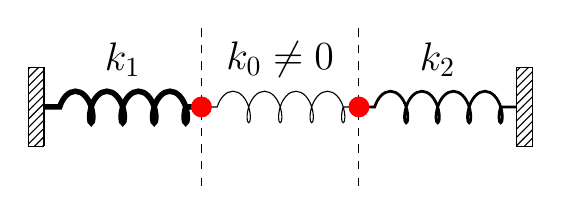
\begin{tikzpicture}
\filldraw[pattern=north east lines] (0,-0.5) -| (-0.2,0.5) -| (0,-0.5);
\filldraw[pattern=north east lines] (6,-0.5) -| (6.2,0.5) -| (6,-0.5);
\draw[Spring, line width=2] (0,0) -- (2,0);
\draw[Spring, thin] (2,0) -- (4,0);
\draw[Spring, line width=1] (4,0) -- (6,0);

\draw [dashed] (2,1) -- (2,-1);
\draw [dashed] (4,1) -- (4,-1);

\draw (2,0) node [fill=red,circle,scale=0.8] {};
\draw (4,0) node [fill=red,circle,scale=0.8] {};

\Large
\draw (1,0.6) node [] {$k_1$};
\draw (3,0.6) node [] {$k_0 \neq 0$};
\draw (5,0.6) node [] {$k_2$};
\end{tikzpicture}
}}

\subfloat[Uncoupled equilibrium]{\scalebox{0.9}{
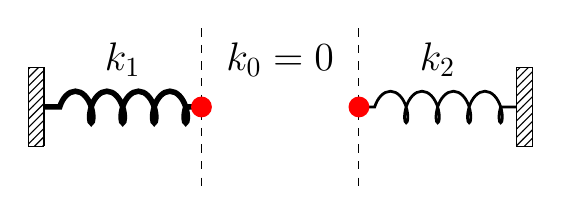
\begin{tikzpicture}
\filldraw[pattern=north east lines] (0,-0.5) -| (-0.2,0.5) -| (0,-0.5);
\filldraw[pattern=north east lines] (6,-0.5) -| (6.2,0.5) -| (6,-0.5);
\draw[Spring, line width=2] (0,0) -- (2,0);
%\draw[Spring, thin] (2,0) -- (4,0);
\draw[Spring, line width=1] (4,0) -- (6,0);

\draw [dashed] (2,1) -- (2,-1);
\draw [dashed] (4,1) -- (4,-1);

\draw (2,0) node [fill=red,circle,scale=0.8] {};
\draw (4,0) node [fill=red,circle,scale=0.8] {};

\Large
\draw (1,0.6) node [] {$k_1$};
\draw (3,0.6) node [] {$k_0 = 0$};
\draw (5,0.6) node [] {$k_2$};
\end{tikzpicture}
}}}

\makebox[\textwidth][c]{
\subfloat[Uncoupled left oscillation]{\scalebox{0.9}{
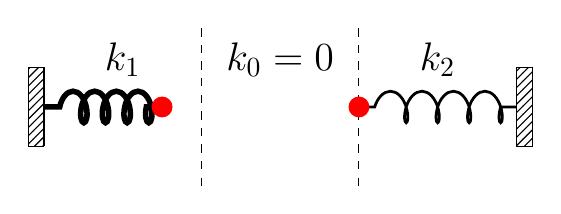
\begin{tikzpicture}
\filldraw[pattern=north east lines] (0,-0.5) -| (-0.2,0.5) -| (0,-0.5);
\filldraw[pattern=north east lines] (6,-0.5) -| (6.2,0.5) -| (6,-0.5);
\draw[Spring, line width=2] (0,0) -- (1.5,0);
%\draw[Spring, thin] (2,0) -- (4,0);
\draw[Spring, line width=1] (4,0) -- (6,0);

\draw [dashed] (2,1) -- (2,-1);
\draw [dashed] (4,1) -- (4,-1);

\draw (1.5,0) node [fill=red,circle,scale=0.8] {};
\draw (4,0) node [fill=red,circle,scale=0.8] {};

\Large
\draw (1,0.6) node [] {$k_1$};
\draw (3,0.6) node [] {$k_0 = 0$};
\draw (5,0.6) node [] {$k_2$};
\end{tikzpicture}
}}

\subfloat[Uncoupled right oscillation]{\scalebox{0.9}{
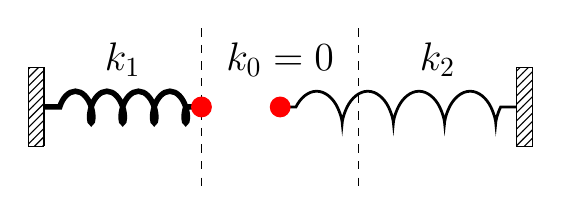
\begin{tikzpicture}
\filldraw[pattern=north east lines] (0,-0.5) -| (-0.2,0.5) -| (0,-0.5);
\filldraw[pattern=north east lines] (6,-0.5) -| (6.2,0.5) -| (6,-0.5);
\draw[Spring, line width=2] (0,0) -- (2,0);
%\draw[Spring, thin] (2,0) -- (4,0);
\draw[Spring, line width=1] (3,0) -- (6,0);

\draw [dashed] (2,1) -- (2,-1);
\draw [dashed] (4,1) -- (4,-1);

\draw (2,0) node [fill=red,circle,scale=0.8] {};
\draw (3,0) node [fill=red,circle,scale=0.8] {};

\Large
\draw (1,0.6) node [] {$k_1$};
\draw (3,0.6) node [] {$k_0 = 0$};
\draw (5,0.6) node [] {$k_2$};
\end{tikzpicture}
}}}
\caption{Mechanical example showing weak and zero coupling between the masses. This provides an analogy to the wide slab approximation of an asymmetric magnetic slab, in which case the interfaces on each side of the slab oscillate independently.}
\label{fig: wide slab mechanical analogy}
\end{figure}

\subsection{Incompressible Approximation} \label{sec: CSAR incomp}

If the plasma in each region is incompressible, the sound speeds become unbounded, so that $m_j \approx k$ for $j = 0,1,2$. Under this approximation, the CSAR for quasi-sausage modes (top) and quasi-kink modes (bottom) reduces to
\begin{align}
R_A &= \left(\substack{- \\ +}\right) \frac{\rho_1}{\rho_2} \left[ \frac{(k^2v_\textrm{A}^2-\omega^2)k\frac{\rho_0}{\rho_1}-\omega^2k \left(\hspace{-0.07in}\begin{matrix} &\coth \\ &\tanh \end{matrix}\right)(kx_0)}{(k^2v_\textrm{A}^2-\omega^2)k\frac{\rho_0}{\rho_2}-\omega^2k \left(\hspace{-0.07in}\begin{matrix} &\coth \\ &\tanh \end{matrix}\right)(kx_0)} \right].
\end{align}
These equations have solutions for $v_A$ given by
\begin{equation}
v_\textrm{A}^2 = \frac{\omega^2}{k^2} \left[ 1 + \left( \frac{R_A \frac{\rho_2}{\rho_0} \left(\substack{+ \\ -}\right) \frac{\rho_1}{\rho_0}}{R_A \left(\substack{+ \\ -}\right) 1} \right) \left(\hspace{-0.07in}\begin{matrix} &\coth \\ &\tanh \end{matrix}\right) (kx_0)\right].
\end{equation}

\subsection{Low-Beta Approximation} \label{sec: CSAR low-beta}

Plasma beta, $\beta = 2\mu_0p_0/B_0^2$, is a non-dimensional parameter defined as the ratio of plasma pressure to magnetic pressure. For a low-beta plasma, where the magnetic pressure dominates the plasma pressure, the Alfv\'{e}n speed, $v_\textrm{A}$, dominates the internal sound speed, $c_0$, so that $m_0^2 \approx k^2-\omega^2/v_\textrm{A}^2$. For waves with phase speed much less than the Alfv\'{e}n speed, a further approximation of $m_0^2 \approx k^2$ can be made, in which case the CSAR for quasi-sausage modes (top) and quasi-kink modes (bottom) reduces to
\begin{align}
R_A &= \left(\substack{- \\ +}\right) \frac{\rho_1m_2}{\rho_2m_1} \left[ \frac{(k^2v_\textrm{A}^2-\omega^2)m_1\frac{\rho_0}{\rho_1}-\omega^2k \left(\hspace{-0.07in}\begin{matrix} &\coth \\ &\tanh \end{matrix}\right)(kx_0)}{(k^2v_\textrm{A}^2-\omega^2)m_2\frac{\rho_0}{\rho_2}-\omega^2k \left(\hspace{-0.07in}\begin{matrix} &\coth \\ &\tanh \end{matrix}\right)(kx_0)} \right].
\end{align}
These equations can be solved for $v_A$ to give
\begin{equation}
v_\textrm{A}^2 = \frac{\omega^2}{k^2} \left[1 + k \left( \frac{ \frac{\rho_1}{\rho_0m_1} \left(\substack{+ \\ -}\right) R_A\frac{\rho_2}{\rho_0m_2}}{1 \left(\substack{+ \\ -}\right) R_A} \right) \left(\hspace{-0.07in}\begin{matrix} &\coth \\ &\tanh \end{matrix}\right) (kx_0)\right].
\end{equation}


%BELOW APPROXIMATION DOES NOT RETAIN MAGNETIC FIELD, SO IS WORTHLESS, PROBABLY.

%\subsection{Approximately Equal External Parameters} \label{sec: approx equal parameters}
%If the parameters of the non-magnetised external regions agree to first order approximation, the dispersion relation for magneto-acoustic waves along an asymmetric slab reduces to
%\begin{align}
%&\Lambda_0(\Lambda_1+\Lambda_2)+2\Lambda_1\Lambda_2\tau_0=0, \label{DR saus} \\
%&\Lambda_0(\Lambda_1+\Lambda_2)+2\Lambda_1\Lambda_2\frac{1}{\tau_0}=0, \label{DR kink}
%\end{align}
%for quasi-sausage and quasi-kink modes, respectively. Manipulation of equation~\eqref{DR saus} yields
%\begin{align}
%\Lambda_0\Lambda_1+\Lambda_1\Lambda_2\tau_0&=-(\Lambda_0\Lambda_2+\Lambda_1\Lambda_2\tau_0), \\
%\implies
%\Lambda_1(\Lambda_0+\Lambda_2\tau_0)&=-\Lambda_2(\Lambda_0+\Lambda_1\tau_0), \\
%\implies \frac{\Lambda_0+\Lambda_1\tau_0}{\Lambda_0+\Lambda_2\tau_0}&=-\frac{\Lambda_1}{\Lambda_2}=-\frac{\rho_1m_2}{\rho_2m_1}.
%\end{align}
%Similar manipulation of equation~\eqref{DR kink} yields
%\begin{equation}
%\frac{\Lambda_0\tau_0+\Lambda_1}{\Lambda_0\tau_0+\Lambda_2}=-\frac{\Lambda_1}{\Lambda_2}=-\frac{\rho_1m_2}{\rho_2m_1}.
%\end{equation}
%If the conditions on either side of the slab are equal to first order approximation, the cross-slab amplitude ratio reduces to
%\begin{equation}
%R_A=-\frac{\rho_1m_2}{\rho_2m_1}, \label{cross-slab ratio approx saus}
%\end{equation}
%for quasi-sausage modes, and
%\begin{equation}
%R_A=\frac{\rho_1m_2}{\rho_2m_1}, \label{cross-slab ratio approx kink}
%\end{equation}
%for quasi-kink modes.


\begin{figure}
\makebox[\textwidth][c]{
\subfloat[]{\scalebox{0.9}{
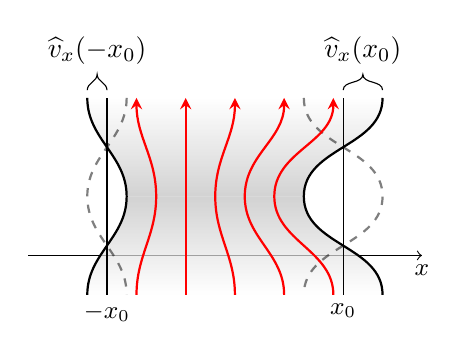
\begin{tikzpicture}
\draw [->] (1,0) -- (6,0);

\shade[bottom color=lightgray,top color=white, opacity=0.7] (1.75,2) to [out=-90,in=90] (2.25,0.75) to (4.5,0.75) to [out=90,in=-90] (5.5,2) to (1.75,2);

\shade[bottom color=white,top color=lightgray, opacity=0.7] (2.25,0.75) to (4.5,0.75) to [out=-90,in=90] (5.5,-0.5) to (1.75,-0.5) to [out=90,in=-90] (2.25,0.75);

\draw [thick] (1.75,2) to [out=-90,in=90] (2.25,0.75) to [out=-90,in=90] (1.75,-0.5);
\draw [thick, dashed, opacity=0.5] (4.5,2) to [out=-90,in=90] (5.5,0.75) to [out=-90,in=90] (4.5,-0.5);

\draw [thick, red, -stealth] (2.375,-0.5) to [out=90,in=-90] (2.625, 0.75) to [out=90,in=-90] (2.375,2);
\draw [thick, red, -stealth] (3,-0.5) to [out=90,in=-90] (3, 0.75) to [out=90,in=-90] (3,2);
\draw [thick, red, -stealth] (3.625,-0.5) to [out=90,in=-90] (3.375, 0.75) to [out=90,in=-90] (3.625,2);
\draw [thick, red, -stealth] (4.25,-0.5) to [out=90,in=-90] (3.75, 0.75) to [out=90,in=-90] (4.25,2);
\draw [thick, red, -stealth] (4.875,-0.5) to [out=90,in=-90] (4.125, 0.75) to [out=90,in=-90] (4.875,2);

\draw [thick, dashed, opacity=0.5] (2.25,2) to [out=-90,in=90] (1.75,0.75) to [out=-90,in=90] (2.25,-0.5);
\draw [thick] (5.5,2) to [out=-90,in=90] (4.5,0.75) to [out=-90,in=90] (5.5,-0.5);

% % % % % % % % % % % % % % % % % % % % % % % % % %

%\draw [->] (0,0) -- (0,2);

%\node at (1,1) {$\rho_1$};
%\node at (6,1) {$\rho_2$};
%\node [right] at (2.95,1.3) {$\rho_0$};

\draw [-] (1.75, 2.1) to [out=90, in=-90] (1.875, 2.3) to [out=-90, in=90] (2, 2.1);
\draw [-] (5, 2.1) to [out=90, in=-90] (5.25, 2.3) to [out=-90, in=90] (5.5, 2.1);

\node [above] at (1.875,2.3) {$\widehat{v}_x(-x_0)$};
\node [above] at (5.25, 2.3) {$\widehat{v}_x(x_0)$};

\small
\node [below] at (2,-0.5) {$-x_0$};
\node [below] at (5,-0.5) {$x_0$};

%\node [left] at (0,2) {$z$};
\node [below] at (6,0) {$x$};
\draw [-] (2,-0.5) -- (2,2);
\draw [-] (5,-0.5) -- (5,2);
\end{tikzpicture}
}}


\subfloat[]{\scalebox{0.9}{
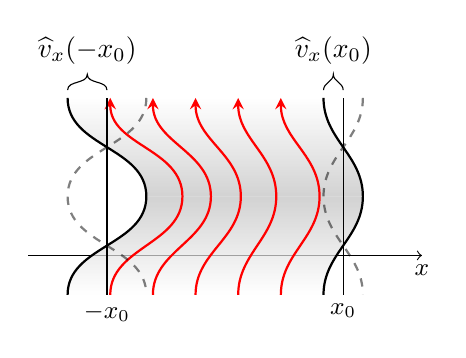
\begin{tikzpicture}
\draw [->] (1,0) -- (6,0);

\shade[bottom color=lightgray,top color=white, opacity=0.7] (1.5,2) to [out=-90,in=90] (2.5,0.75) to (5.25,0.75) to [out=90,in=-90] (4.75,2) to (1.5,2);

\shade[bottom color=white,top color=lightgray, opacity=0.7] (2.5,0.75) to (5.25,0.75) to [out=-90,in=90] (4.75,-0.5) to (1.5,-0.5) to [out=90,in=-90] (2.5,0.75);

\draw [thick] (1.5,2) to [out=-90,in=90] (2.5,0.75) to [out=-90,in=90] (1.5,-0.5);
\draw [thick] (4.75,2) to [out=-90,in=90] (5.25,0.75) to [out=-90,in=90] (4.75,-0.5);

%\draw [thick, red, -stealth] (2.0417,-0.5) to [out=90,in=-90] (2.9583, 0.75) to [out=90,in=-90] (2.0417,2);
%\draw [thick, red, -stealth] (2.5833,-0.5) to [out=90,in=-90] (3.4167, 0.75) to [out=90,in=-90] (2.5833,2);
%\draw [thick, red, -stealth] (3.125,-0.5) to [out=90,in=-90] (3.875, 0.75) to [out=90,in=-90] (3.125,2);
%\draw [thick, red, -stealth] (3.6667,-0.5) to [out=90,in=-90] (4.3333, 0.75) to [out=90,in=-90] (3.6667,2);
%\draw [thick, red, -stealth] (4.2083,-0.5) to [out=90,in=-90] (4.7917, 0.75) to [out=90,in=-90] (4.2083,2);

\draw [thick, red, -stealth] (2.0417,-0.5) to [out=90,in=-90] (2.9583, 0.75) to [out=90,in=-90] (2.0417,2);
\draw [thick, red, -stealth] (2.5833,-0.5) to [out=90,in=-90] (3.32, 0.75) to [out=90,in=-90] (2.5833,2);
\draw [thick, red, -stealth] (3.125,-0.5) to [out=90,in=-90] (3.7, 0.75) to [out=90,in=-90] (3.125,2);
\draw [thick, red, -stealth] (3.6667,-0.5) to [out=90,in=-90] (4.15, 0.75) to [out=90,in=-90] (3.6667,2);
\draw [thick, red, -stealth] (4.2083,-0.5) to [out=90,in=-90] (4.7, 0.75) to [out=90,in=-90] (4.2083,2);

\draw [thick, dashed, opacity=0.5] (2.5,2) to [out=-90,in=90] (1.5,0.75) to [out=-90,in=90] (2.5,-0.5);
\draw [thick, dashed, opacity=0.5] (5.25,2) to [out=-90,in=90] (4.75,0.75) to [out=-90,in=90] (5.25,-0.5);

% % % % % % % % % % % % % % % % % % % % % % % % % %

\draw [-] (1.5, 2.1) to [out=90, in=-90] (1.75, 2.3) to [out=-90, in=90] (2., 2.1);
\draw [-] (4.75, 2.1) to [out=90, in=-90] (4.875, 2.3) to [out=-90, in=90] (5., 2.1);

\node [above] at (1.75,2.3) {$\widehat{v}_x(-x_0)$};
\node [above] at (4.875, 2.3) {$\widehat{v}_x(x_0)$};

\small
\node [below] at (2,-0.5) {$-x_0$};
\node [below] at (5,-0.5) {$x_0$};

%\node [left] at (0,2) {$z$};
\node [below] at (6,0) {$x$};
\draw [-] (2,-0.5) -- (2,2);
\draw [-] (5,-0.5) -- (5,2);
\end{tikzpicture}
}}}


\makebox[\textwidth][c]{
\subfloat[]{\scalebox{0.9}{
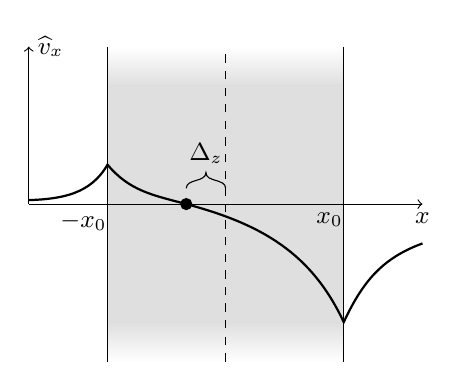
\begin{tikzpicture}
\path [fill=lightgray, opacity=0.5] (2,-1.5) -- (2,1.5) -- (5,1.5) -- (5,-1.5) -- (2,-1.5);

\shade[bottom color=white,top color=lightgray, opacity=0.5] (2,-2) to (5,-2) to (5,-1.5) to (2,-1.5) to (2,-2);

\shade[top color=white,bottom color=lightgray, opacity=0.5] (2,2) to (5,2) to (5,1.5) to (2,1.5) to (2,2);

\draw [-] (2,-2) -- (2,2);
\draw [-] (5,-2) -- (5,2);

%\draw [ultra thick, red, -stealth,opacity=0.7] (2.5,-1.5) -- (2.5,2);
%\draw [ultra thick, red, path fading=south, opacity=0.5] (2.5,-2) -- (2.5,-1.5);
%\draw [ultra thick, red, -stealth,opacity=0.7] (3,-1.5) -- (3,2);
%\draw [ultra thick, red, path fading=south,opacity=0.5] (3,-2) -- (3,-1.5);
%\draw [ultra thick, red, -stealth,opacity=0.7] (3.5,-1.5) -- (3.5,2);
%\draw [ultra thick, red, path fading=south,opacity=0.5] (3.5,-2) -- (3.5,-1.5);
%\draw [ultra thick, red, -stealth,opacity=0.7] (4,-1.5) -- (4,2);
%\draw [ultra thick, red, path fading=south,opacity=0.5] (4,-2) -- (4,-1.5);
%\draw [ultra thick, red, -stealth,opacity=0.7] (4.5,-1.5) -- (4.5,2);
%\draw [ultra thick, red, path fading=south,opacity=0.5] (4.5,-2) -- (4.5,-1.5);

%\draw [thick] (0,0.025) to [out=0, in=-178] (1.2, 0.05) to [out=2, in=-120] (2,0.5) to [out=-50, in=165] (3,0) to [out=-15, in=115] (5,-1.5) to [out=65, in=-170] (7,-0.2);

\draw [thick] (1, 0.05) to [out=2, in=-120] (2,0.5) to [out=-50, in=165] (3,0) to [out=-15, in=115] (5,-1.5) to [out=65, in=-160] (6,-0.5);

\draw [->] (1,0) -- (1,2);
\draw [->] (1,0) -- (6,0);

%\node at (1,1) {$\rho_1$};
%\node at (6,1) {$\rho_2$};
%\node [right] at (2.88,1.3) {$\rho_0$};

\small
\node [below left] at (2.1,0) {$-x_0$};
\node [below left] at (5.1,0) {$x_0$};

\node [right] at (1,2) {$\widehat{v}_x$};
\node [below] at (6,0) {$x$};

\draw [dashed] (3.5,-2) -- (3.5,2);
\draw [fill] (3,0) circle [radius=0.07];
\draw [-] (3, 0.2) to [out=90, in=-90] (3.25, 0.4) to [out=-90, in=90] (3.5, 0.2);
\node [above] at (3.25, 0.4) {$\Delta_z$};
\end{tikzpicture}
}}


\subfloat[]{\scalebox{0.9}{
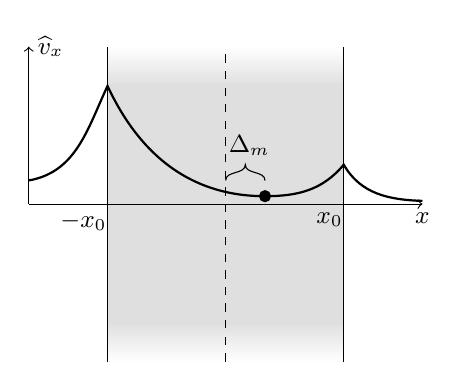
\begin{tikzpicture}
\path [fill=lightgray, opacity=0.5] (2,-1.5) -- (2,1.5) -- (5,1.5) -- (5,-1.5) -- (2,-1.5);

\shade[bottom color=white,top color=lightgray, opacity=0.5] (2,-2) to (5,-2) to (5,-1.5) to (2,-1.5) to (2,-2);

\shade[top color=white,bottom color=lightgray, opacity=0.5] (2,2) to (5,2) to (5,1.5) to (2,1.5) to (2,2);

\draw [-] (2,-2) -- (2,2);
\draw [-] (5,-2) -- (5,2);

%\draw [ultra thick, red, -stealth,opacity=0.7] (2.5,-1.5) -- (2.5,2);
%\draw [ultra thick, red, path fading=south, opacity=0.5] (2.5,-2) -- (2.5,-1.5);
%\draw [ultra thick, red, -stealth,opacity=0.7] (3,-1.5) -- (3,2);
%\draw [ultra thick, red, path fading=south,opacity=0.5] (3,-2) -- (3,-1.5);
%\draw [ultra thick, red, -stealth,opacity=0.7] (3.5,-1.5) -- (3.5,2);
%\draw [ultra thick, red, path fading=south,opacity=0.5] (3.5,-2) -- (3.5,-1.5);
%\draw [ultra thick, red, -stealth,opacity=0.7] (4,-1.5) -- (4,2);
%\draw [ultra thick, red, path fading=south,opacity=0.5] (4,-2) -- (4,-1.5);
%\draw [ultra thick, red, -stealth,opacity=0.7] (4.5,-1.5) -- (4.5,2);
%\draw [ultra thick, red, path fading=south,opacity=0.5] (4.5,-2) -- (4.5,-1.5);

%\draw [thick] (0,0.2) to [out=10, in=245] (2, 1.5) to [out=295, in=180] (4,0.1) to [out=0, in=230] (5,0.5) to [out=300, in=178] (6.2,0.04) to [out=358, in=180] (7,0.02);

\draw [thick] (1,0.3) to [out=10, in=245] (2, 1.5) to [out=295, in=180] (4,0.1) to [out=0, in=230] (5,0.5) to [out=300, in=178] (6,0.04);

\draw [->] (1,0) -- (1,2);
\draw [->] (1,0) -- (6,0);
%
%\node at (1,1) {$\rho_1$};
%\node at (6,1) {$\rho_2$};
%\node [right] at (2.88,1.3) {$\rho_0$};

\small
\node [below left] at (2.1,0) {$-x_0$};
\node [below left] at (5.1,0) {$x_0$};

\node [right] at (1,2) {$\widehat{v}_x$};
\node [below] at (6,0) {$x$};

\draw [dashed] (3.5,-2) -- (3.5,2);
\draw [fill] (4,0.1) circle [radius=0.07];
\draw [-] (3.5, 0.3) to [out=90, in=-90] (3.75, 0.5) to [out=-90, in=90] (4, 0.3);
\node [above] at (3.8, 0.5) {$\Delta_m$};
\end{tikzpicture}
}}}

\caption{(a) and (b) illustrate the difference in amplitude of oscillation on each boundary of the slab for quasi-sausage and quasi-kink modes. (c) and (d) illustrate the shift of minimum perturbation within the slab for quasi-sausage and quasi-kink modes. Both the ratio of the amplitudes and the shift in minimum perturbation can be used as a diagnostic tool.}
\end{figure}


\section{Shift of minimum perturbation}
An additional eigenfunction-based solar magneto-seismology technique uses the shift in the position of minimum wave power from the centre of the slab due to the asymmetry in the external plasma regions.

The position of minimum wave power for a symmetric sausage or kink mode is on the central line of the slab, at $x=0$. We define $\Delta_\textrm{min}$ to be the displacement (from the central line) of the position of minimum wave power inside an asymmetric magnetic slab. For quasi-sausage modes, the value of $\Delta_\textrm{min}$ will be the solution to $\widehat{v}_x(x) = 0$ under the constraint $|x| < x_0$, and for quasi-kink modes, the value of $\Delta_\textrm{min}$ will be the solution to $\textrm{d}\widehat{v}_x (x) / \textrm{d}x = 0$ under the same constraint $|x| < x_0$. The constraint restricts the solutions to being within the slab. 

Firstly, for quasi-sausage modes, using the solution for the transversal velocity amplitude given by Equation~\eqref{vsoln} and the expressions for the variables within given by equation~\eqref{constB C}, the shift of minimum perturbation can be calculated as follows. The solution for the transversal velocity amplitude within the slab is
\begin{equation}
\widehat{v}_x(x) = B\cosh{m_0x}+C\sinh{m_0x} = 0,
\end{equation}
where $B$ is given by equation~\eqref{constB C} and $C$ is arbitrary. This equation is solved to give
\begin{equation}
x = \frac{1}{m_0} \tanh^{-1}\left(-\frac{B}{C}\right). \label{disp of min power saus}
\end{equation}
therefore the shift of minimum perturbation is
\begin{equation}
\Delta_{min} = \frac{1}{m_0}\tanh^{-1}\left(-\frac{(k^2{v_A}^2-\omega^2)m_1\frac{\rho_0}{\rho_1} - \omega^2{m_0}\tanh{m_0x_0}}{(k^2{v_A}^2-\omega^2)m_1\frac{\rho_0}{\rho_1}\tanh{m_0x_0} - \omega^2{m_0}}\right). \label{shift min saus}
\end{equation}
Secondly, for quasi-kink modes, using equations~\eqref{vsoln} and \eqref{constB B} we calculate the shift of minimum perturbation to be
\begin{equation}
\Delta_{min} = \frac{1}{m_0}\coth^{-1}\left(-\frac{(k^2{v_A}^2-\omega^2)m_1\frac{\rho_0}{\rho_1} - \omega^2{m_0}\tanh{m_0x_0}}{(k^2{v_A}^2-\omega^2)m_1\frac{\rho_0}{\rho_1}\tanh{m_0x_0} - \omega^2{m_0}}\right). \label{shift min kink}
\end{equation}

It appears that expressions~\eqref{shift min saus} and~\eqref{shift min kink} for the shift in minimum perturbations depend on the parameters in the slab (subscript~0), the left external plasma (subscript~1), but not on the right external plasma (subscript~2). However, the dependence on the right external plasma is implicit in the determination of the eigenfrequency $\omega$ when solving the dispersion relation \citep{all_etal17}.

The concept of minimum perturbation shift is exclusive to surface modes. The eigenfunctions of surface modes in a magnetic slab depend much more on the plasma parameters, such as the density, than body modes \citep{all_etal17}. This makes intuitive sense given that the energy in a surface mode is localised to the boundaries of the slab whereas the energy in a body mode is largely isolated within the slab. There is a quantifiable shift in the spatial nodes and anti-nodes in body mode perturbations within a slab due to changing external plasma parameters, however it is so small that is would not be an effective observational tool. It is also much more sophisticated because it depends on the number of internal nodes that the particular body mode has, an observation that is yet to be made in solar structures in either slab or tube geometries.

Akin to the amplitude ratio method for solar magneto-seismology prescribed in Section~\ref{sec: CSAR}, we can solve equation~\eqref{shift min saus} or~\eqref{shift min kink} for the Alfv\'{e}n speed, $v_A$, to achieve an approximation for the magnetic field strength of inhomogeneous solar magnetic structures. This can be done either numerically, using an iterative root finding method, or analytically, under an appropriate approximation, as discussed below.


\subsection{Thin slab approximation}
As noted in Section~\ref{sec: CSAR thin slab}, for surface modes, the thin slab limit, that is $kx_0 \ll 1$ implies $m_0x_0 \ll 1$. Since, by definition, $\Delta_{min} < x_0$, then $m_0\Delta_{min} \ll 1$ so that $\tanh{m_0\Delta_{min}} \approx m_0\Delta_{min}$. Firstly, for quasi-sausage modes, Equation~\eqref{shift min saus} can be solved for $v_A$ to give
\begin{equation}
v_A^2 = \frac{\omega^2}{k^2} \left[\frac{\rho_1}{\rho_0m_1}(x_0 + \Delta_{min}) + \frac{1}{1 + (\omega / kc_0)^2} + k^2x_0\Delta_{min}\right].
\end{equation}

For quasi-kink modes in a thin slab, Equation~\eqref{shift min kink} can be solved for $v_A$ to give
\begin{equation}
v_A^2 = \frac{\omega^2}{k^2}\left[\frac{-b \pm \sqrt{b^2 - 4ac}}{2a}\right],
\end{equation}
where
\begin{align}
a &= m_1\frac{\rho_0}{\rho_1}(k^2c_0^2 - \omega^2)(x_0 + \Delta_{min}), \\
b &= -m_1\frac{\rho_0}{\rho_1}(2k^2c_0^2 - \omega^2)(x_0 + \Delta_{min}) - (k^2c_0^2 - \omega^2), \\
c &= c_0^2m_1\frac{\rho_0}{\rho_1}(x_0 + \Delta_{min}) + c_0^2 + \omega^2x_0\Delta_{min}.
\end{align}


\subsection{Wide slab approximation}
The concept of minimum perturbation shift is ill-defined under the wide slab approximation. In the wide slab approximation, each interface oscillated independently at its own eigenfrequency. Therefore the nomenclature of quasi-sausage and quasi-kink mode breaks down. In the wide slab limit, the eigenfunctions have no local minimum in the slab, instead the perturbations are evanescent away from the interface that the oscillation is localised, therefore there is no local minimum in wave power within the slab.


\subsection{Incompressible approximation}
When the plasma is incompressible, the sound speeds are unbounded, so that $m_j = k$, for $j = 0, 1, 2$. The shift in minimum perturbation for a quasi-sausage mode (top) and quasi-kink (bottom) in an incompressible slab is
\begin{equation}
\Delta_{min} = \frac{1}{k}\left(\hspace{-0.07in}\begin{matrix} &\tanh^{-1} \\ &\coth^{-1} \end{matrix}\right)\left(-\frac{(k^2{v_A}^2-\omega^2)\frac{\rho_0}{\rho_1} - \omega^2\tanh{kx_0}}{(k^2{v_A}^2-\omega^2)\frac{\rho_0}{\rho_1}\tanh{kx_0} - \omega^2}\right),
\end{equation}
which can be solved for $v_A$ to give
\begin{equation}
v_A^2 = \frac{\omega^2}{k^2}\left[1 + \frac{\rho_1}{\rho_0}\left(\hspace{-0.07in}\begin{matrix} &\tanh \\ &\coth \end{matrix}\right)(k(x_0 + \Delta_{min}))\right].
\end{equation}


\subsection{Low-beta approximation}
In a low-beta plasma, the shift in minimum perturbation for a quasi-sausage mode (top) and quasi-kink (bottom) is given by
\begin{equation}
\Delta_{min} = \frac{1}{k}\left(\hspace{-0.07in}\begin{matrix} &\tanh^{-1} \\ &\coth^{-1} \end{matrix}\right)\left(-\frac{(k^2{v_A}^2-\omega^2)m_1\frac{\rho_0}{\rho_1} - \omega^2k\tanh{kx_0}}{(k^2{v_A}^2-\omega^2)m_1\frac{\rho_0}{\rho_1}\tanh{kx_0} - \omega^2k}\right),
\end{equation}
which can be solved for $v_A$ to give
\begin{equation}
v_A^2 = \frac{\omega^2}{k^2}\left[1 + \frac{k\rho_1}{m_1\rho_0}\left(\hspace{-0.07in}\begin{matrix} &\tanh \\ &\coth \end{matrix}\right)(k(x_0 + \Delta_{min}))\right].
\end{equation}

\newgeometry{margin=1cm} % modify this if you need even more space
\begin{landscape}


\begin{table}
\caption{Magneto-seismological application using the amplitude ratio, $R_A$, to approximate the Alfv\'{e}n speed, $v_A$, dependant on the type of mode observed.}
\begin{tabular}{llccc}
  \toprule
Type & Mode & \multicolumn{3}{c}{Approximation of $k^2v_A^2 / \omega^2$ using amplitude ratio, $R_A$} \\
\cmidrule(lr){3-5}
	 &	    & \multicolumn{1}{c}{Thin slab} & \multicolumn{1}{c}{Incompressible} & \multicolumn{1}{c}{Low-beta} \\
  \midrule
\multirow{2}{*}{Surface} & Quasi-sausage & $ 1 + \frac{1}{x_0}\left(\frac{R_A\frac{\rho_2}{\rho_0m_2} + \frac{\rho_1}{\rho_0m_1}}{R_A + 1}\right) $ & $ 1 + \left( \frac{R_A \frac{\rho_2}{\rho_0} + \frac{\rho_1}{\rho_0}}{R_A + 1} \right) \coth{kx_0} $ & $ 1 + k \left( \frac{ \frac{\rho_1}{\rho_0m_1} + R_A\frac{\rho_2}{\rho_0m_2}}{1 + R_A} \right) \coth{kx_0} $ \\
						   & Quasi-kink	   & $ 1 + k^2x_0\left(\frac{R_A\frac{\rho_2}{\rho_0m_2} - \frac{\rho_1}{\rho_0m_1}}{R_A - 1}\right) $ & $ 1 + \left( \frac{R_A \frac{\rho_2}{\rho_0} - \frac{\rho_1}{\rho_0}}{R_A - 1} \right) \tanh{kx_0} $ & $ 1 + k \left( \frac{ \frac{\rho_1}{\rho_0m_1} - R_A\frac{\rho_2}{\rho_0m_2}}{1 - R_A} \right) \tanh{kx_0} $ \\
\multirow{2}{*}{Body}    & Quasi-sausage & N/A & N/A & N/A \\
						   & Quasi-kink	   & N/A & N/A & N/A \\
  \bottomrule
\end{tabular} \label{table: amp ratio}
\end{table}



\begin{table}
\caption{Magneto-seismological application using the minimum perturbation shift, $\Delta_{min}$, to approximate the Alfv\'{e}n speed, $v_A$, dependant on the type of mode observed.}
\begin{tabular}{llccc}
  \toprule
Type & Mode & \multicolumn{3}{c}{Approximation of $k^2v_A^2 / \omega^2$ using minimum perturbation shift, $\Delta_{min}$} \\
\cmidrule(lr){3-5}
	 &	    & Thin slab & Incompressible & Low-beta \\
  \midrule
\multirow{2}{*}{Surface} & Quasi-sausage & $ \frac{\rho_1}{\rho_0m_1}(x_0 + \Delta_{min}) + \frac{1}{1 + (\omega / kc_0)^2} + k^2x_0\Delta_{min} $ & $ 1 + \frac{\rho_1}{\rho_0}\tanh{k(x_0 + \Delta_{min})} $ & $ 1 + \frac{k\rho_1}{m_1\rho_0}\tanh{k(x_0 + \Delta_{min})} $ \\
						   & Quasi-kink	   & $\frac{-b \pm \sqrt{b^2 - 4ac}}{2a}$, defined in text & $ 1 + \frac{\rho_1}{\rho_0}\coth{k(x_0 + \Delta_{min})} $ & $ 1 + \frac{k\rho_1}{m_1\rho_0}\coth{k(x_0 + \Delta_{min})} $ \\
\multirow{2}{*}{Body}    & Quasi-sausage & N/A & N/A & N/A \\
						   & Quasi-kink	   & N/A & N/A & N/A \\
  \bottomrule
\end{tabular} \label{table: shift in min pert}
\end{table}

\end{landscape}
\restoregeometry

\section{Discussion}

Presented above are the concepts of the amplitude ratio and the shift in minimum perturbation, both of which can either be solved for the Alfv\'{e}n speed either numerically, for a given set of observed parameters, or analytically, under and appropriate approximation. A summary of the analytical procedure for estimating the Alfv\'{e}n speed, $v_A$, within an magnetic slab is given in Tables~\ref{table: amp ratio} and~\ref{table: shift in min pert}, using the amplitude method and the shift in minimum perturbation methods, respectively. From this, an estimate of the magnetic field strength can be made. In practice, a numerical procedure would be relatively simple and computationally cheap by making use of a standard root finding method once the observed parameters have been substituted.

The next step along the development of this method is to determine whether magneto-acoustic waves can be set up in an asymmetric waveguide within the characteristic lifetime of such a structure in the solar atmosphere. This can be established analytically (for linear waves with simple initial conditions) and numerically (for nonlinear waves with more sophisticated initial conditions), and will be the subject of future work. Further, a more realistic system, including magnetic fields in the external plasmas, would allow for better application to solar waveguides.


%%%%%%%%%%%%%%%%%%%%%%%%%%%%%%%%%%%%%%%%%%%%%%%%%%%%%%%%%%%%%%

\bibliographystyle{spr-mp-sola}
\bibliography{Bibliography}

\end{article} 
\end{document}